%(BEGIN_QUESTION)
% Copyright 2006, Tony R. Kuphaldt, released under the Creative Commons Attribution License (v 1.0)
% This means you may do almost anything with this work of mine, so long as you give me proper credit

Når du bruker termoelementkalibrator (simulator), der du kun setter en temperatur som skal simuleres, er det da viktig å bruke korrekt termoelement- eller forlengelsesledning mellom kalibrator og transmitter, eller er ledningstypen irrelevant?

$$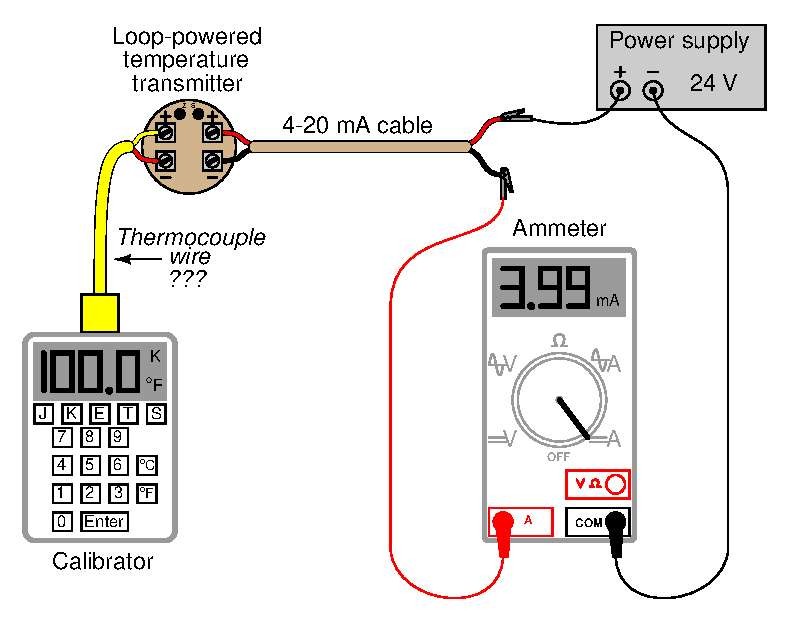
\includegraphics[width=15.5cm]{i00396x01.eps}$$

Begrunn svaret med utgangspunkt i skjøter mellom ulike metaller og kompenseringskretser i både kalibrator og transmitter.

\underbar{file i00396}
%(END_QUESTION)





%(BEGIN_ANSWER)

Ideelt kan vi bruke hvilken som helst ledningstype så lenge både kalibrator og transmitter har nøyaktig samme temperatur. Hvis temperaturene ikke er like, må vi bruke riktig termoelementledning (eller forlengelsesledning) mellom kalibrator og instrument.

%(END_ANSWER)





%(BEGIN_NOTES)

Selv med dette er det anbefalt å bruke samme type ledning som termoelementet, i tilfelle tilkoblingspunktene på de to instrumentene ikke er termisk utjevnet.

Det anbefales også å la kalibratoren få samme temperatur som transmitteren, for å redusere feilrisiko når to sett referanseskjøter (og kompenseringskretser) arbeider ved ulike temperaturer.

%INDEX% Measurement, temperature: thermocouple calibrator (simulator)

%(END_NOTES)
